%!TEX root = ../template.tex
%%%%%%%%%%%%%%%%%%%%%%%%%%%%%%%%%%%%%%%%%%%%%%%%%%%%%%%%%%%%%%%%%%%
%% chapter5.tex
%% UNIPD thesis document file
%%
%% Chapter with introduction
%%%%%%%%%%%%%%%%%%%%%%%%%%%%%%%%%%%%%%%%%%%%%%%%%%%%%%%%%%%%%%%%%%%

\typeout{NT FILE chapter5.tex}%

\chapter{Progettazione e Implementazione di un Sistema di Streaming Audio}
\label{cha:streamingaudio}

\prependtographicspath{{Chapters/Figures/Covers/}}

Le soluzioni commerciali proposte da marchi rinomati come Sonos, Marshall e Bose richiederebbero l'installazione di collegamenti cablati in ogni sezione dell'edificio, rappresentando inoltre una scelta onerosa in termini di costi. Inoltre, la centralizzazione di questi sistemi da un singolo server si è dimostrata problematica. Per superare queste sfide, viene proposto un approccio wireless innovativo, in cui un server primario è incaricato di distribuire file audio pre registrati ai diversi client presenti nella rete.

Il sistema proposto deve soddisfare tre requisiti fondamentali. Primo, è necessaria una stretta dipendenza tra le librerie del server primario e dei client. Secondo, occorre una connessione internet robusta o una rete locale, con il server principale configurato con un indirizzo IP statico. Terzo, l'intera architettura deve essere economicamente vantaggiosa, semplificando sia l'implementazione che la manutenzione.

Per realizzare questo progetto, si è scelto di utilizzare il Raspberry Pi, un microcomputer con il supporto del sistema operativo Linux. Dopo ulteriori ricerche, è stata selezionata la versione DietPi, basata su Debian, preferendola ad altre versioni con \gls{gui}. Sono stati quindi considerati due possibili approcci di implementazione: uno basato su Balena Sound con sistema operativo Balena e l'altro impiegando i server Mopidy e Snapcast su DietPi.

Questa introduzione pone le basi per una discussione dettagliata su come realizzare un sistema di comunicazione audio efficiente e scalabile in un ambiente educativo distribuito, affrontando sfide pratiche con soluzioni tecnologiche innovative.

\section{Architettuera del Sistema}
\noindent

Il progetto richiede un ecosistema completo che permetta di trasformare un tradizionale sistema di altoparlanti cablati in un sistema wireless. Gli altoparlanti devono poter comunicare con il server principale, che consente la trasmissione di musica o file audio richiesti dal cliente. Per implementare questo sistema, è stato scelto un hardware compatibile con Linux, come il Raspberry Pi (nello specifico il Zero 2w), utilizzando il sistema operativo DietPi per ottimizzare l’uso della memoria cache della CPU e della memoria Ram.

Snapcast è stato installato sia sul server che sui client, permettendo una trasmissione audio sincronizzata multi-room tra i dispositivi. \cite{snapcast}

Per consentire l’accesso remoto al server e la gestione della riproduzione musicale, è stato implementato Mopidy \cite{mopidy}, un server musicale versatile. In quale offre diverse estensioni, come Mopidy-File, Mopidy-Iris e Mopidy-Mobile, che facilitano l’accesso e la gestione dei file musicali presenti nella directory locale e/o server designata. Insieme a Mopidy, è stato installato anche \gls{mpd} per creare un ambiente di riproduzione musicale virtuale, che consente l’accesso remoto attraverso interfacce come Iris (frontend) o \gls{mobile}. Con queste estensioni, è possibile eseguire i comandi basici come riproduzione, mettere in pausa e regolare il volume. Il controllo del volume dell’intero gruppo di altoparlanti è possibile solo se Snapcast è abilitato e in esecuzione come servizio.

\begin{figure}[h]
    \centering
    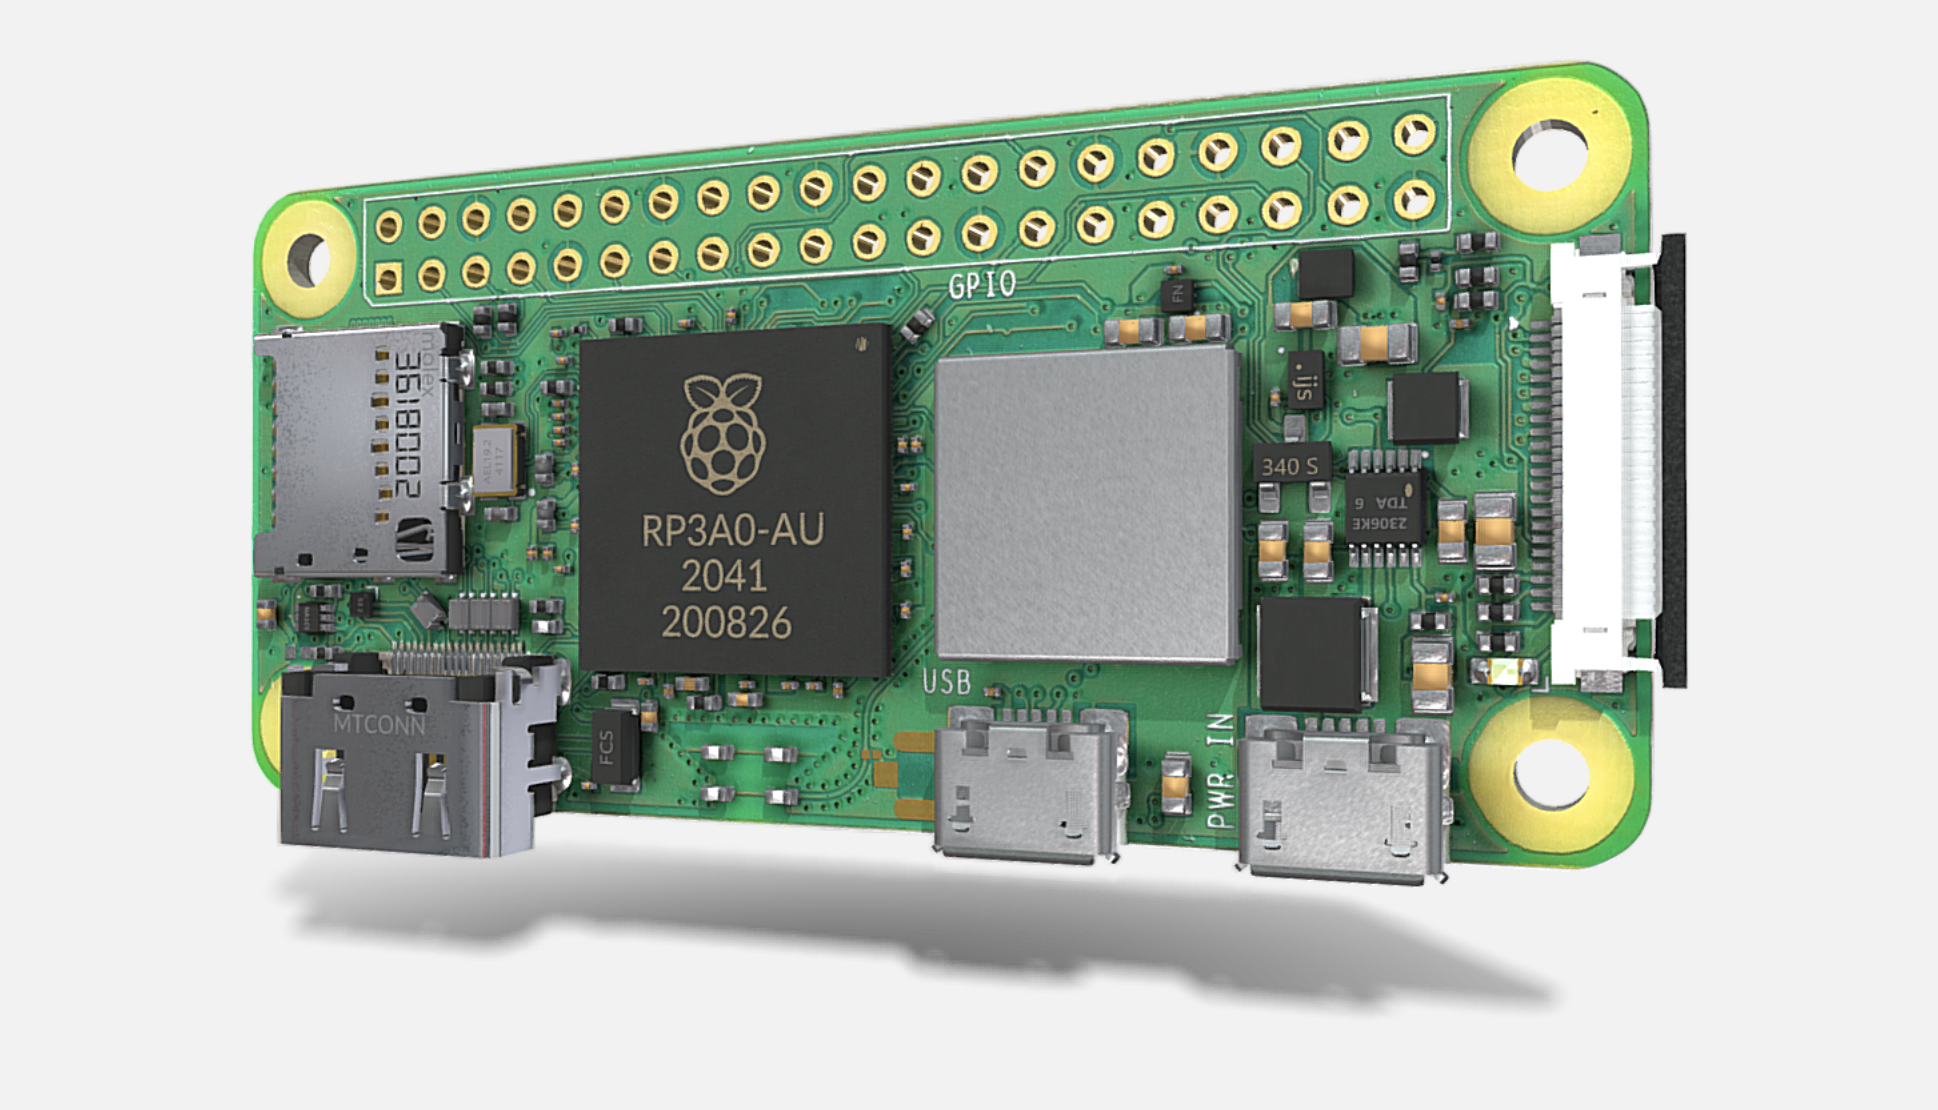
\includegraphics[width=0.5\textwidth]{Chapters/Figures/3d_render_2w.png}
    \caption{\small Raspberry Pi Zero 2W.} 
    \label{fig:zero2w_3d_render}
\end{figure}

\begin{comment}

\begin{figure}[h]
    \centering
    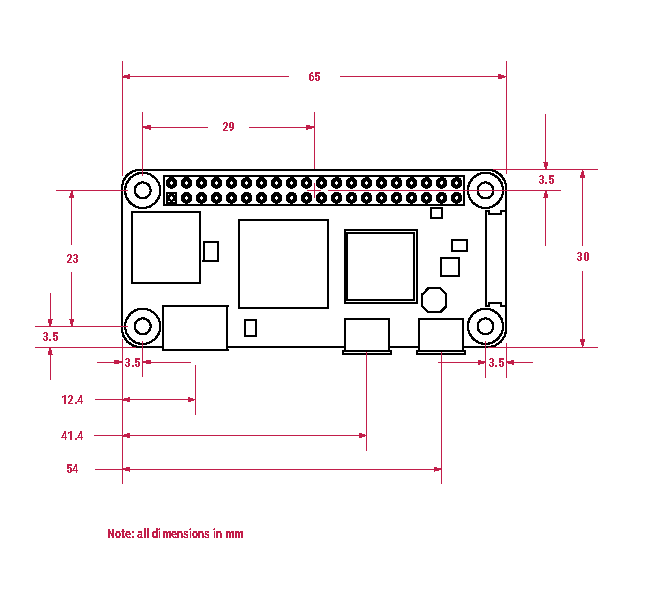
\includegraphics[width=0.6\textwidth]{Chapters/Figures/mechanical_scheme_2w.pdf}
    \caption{\small Raspberry Pi Zero 2w mechanical scheme. \cite{parallax}} 
    \label{fig:zero2w_mechanical_scheme}
\end{figure}

\end{comment}

\section{Stack Software e Componenti}
\noindent

Snapcast si presenta come una soluzione avanzata per la gestione dell'audio in ambienti multipli.  Si tratta di un sistema client-server progettato specificamente per configurazioni che coinvolgono più stanze, dove la sincronizzazione tra server e client è fondamentale per garantire una riproduzione audio simultanea. È importante notare che Snapcast non è concepito come un player autonomo, ma piuttosto come un'estensione che trasforma un comune player audio in un sistema più complesso, capace di espandere le potenzialità di un semplice Home Theater dalla limitazione di una singola stanza all'intera struttura.

Il funzionamento di Snapcast è particolarmente interessante dal punto di vista tecnico. Il server agisce come punto centrale di raccolta dell'audio, che viene poi distribuito ai vari client connessi. Una caratteristica notevole è la sua flessibilità: il sistema può gestire contemporaneamente più player che trasmettono audio in parallelo al server, e offre la possibilità di raggruppare i client per la riproduzione dello stesso flusso audio. Questa versatilità lo rende particolarmente adatto all'integrazione con sistemi come \gls{mpd} o Mopidy, che rappresentano infatti una delle sue applicazioni più comuni.

\begin{figure}[H]
    \centering
    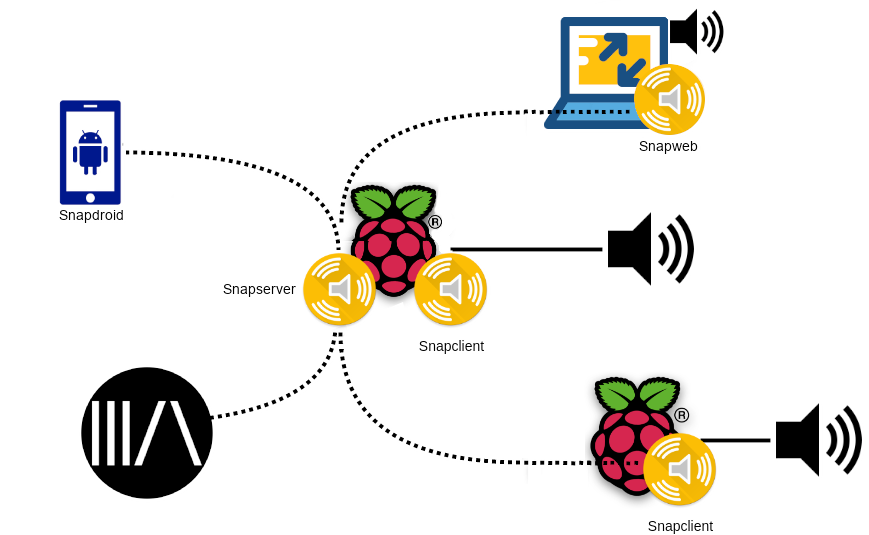
\includegraphics[width=0.5\textwidth]{Chapters/Figures/snapcast_client.png}
    \caption{\small Snapcast muti room audio setup.} 
    \label{fig:snapcast_client}
\end{figure}

Il processo di trasmissione dati in Snapcast è stato accuratamente progettato per garantire efficienza e sincronizzazione. I dati audio vengono inviati sotto forma di frammenti criptati attraverso una connessione \gls{tcp} sicura. Ogni client mantiene una sincronizzazione costante con il server, garantendo così una perfetta coordinazione temporale. Quando i frammenti audio raggiungono il client, vengono prima decodificati e inseriti in un buffer dedicato, per poi essere riprodotti al momento esatto attraverso \gls{api} audio di basso livello, come ALSA. Un aspetto particolarmente sofisticato è la gestione della latenza: il sistema è in grado di correggere eventuali ritardi rimuovendo o duplicando singoli campioni audio per ottimizzare la velocità di riproduzione, con una precisione tale che ogni campione a 48kHz ha una durata di appena 0.02 millisecondi.

Il secondo componente fondamentale del sistema è Mopidy, un'applicazione sviluppata in Python che si distingue per la sua versatilità e facilità d'uso. Può essere eseguita sia in un terminale che in background su qualsiasi computer Linux o Mac connesso alla rete, offrendo una flessibilità notevole nell'implementazione. Mopidy si presenta con un server \gls{http} già pronto all'uso, e grazie all'estensione Mopidy \gls{mpd} , può funzionare anche come server \gls{mpd} completo. Una delle sue caratteristiche più apprezzabili è la vasta gamma di frontend disponibili come estensioni, che permettono di controllare il sistema in modi diversi.

La compatibilità universale di Mopidy con i principali sistemi operativi, unita alla possibilità di controllarlo da qualsiasi dispositivo - che sia un telefono, un tablet o un computer - attraverso il browser web o il client MPD, lo rende una scelta ideale per un sistema di diffusione audio distribuito come quello richiesto dal progetto delle “bolle sonore” dedicato alla ristorazione.

Questa combinazione di Snapcast e Mopidy crea quindi una base solida e flessibile per l'implementazione di un sistema audio multi-room efficiente e affidabile, capace di soddisfare le esigenze specifiche del progetto mantenendo al contempo un'elevata qualità di riproduzione e sincronizzazione.

\section{Implementazione del Backend}
\noindent


L'implementazione del backend concerne la configurazione e lo sviluppo dei componenti server del sistema di streaming. Il server centrale, costruito su Raspberry Pi, ospita sia Snapserver che Mopidy, offrendo i servizi necessari per la gestione e la distribuzione dei flussi audio ai client.

\subsection{Configurazione del Server}

Il server principale, posizionato fisicamente nella sala server, richiede una configurazione specifica dell'indirizzo IP statico per garantire una connessione stabile e affidabile. Il sistema è stato configurato con Mopidy per la gestione delle sorgenti audio e della libreria musicale. Il file di configurazione di Mopidy è stato personalizzato per ottimizzare la gestione dell'audio:

\begin{table}[H]
    \begin{minipage}{0.8\textwidth}
      \begin{verbatim}
        [audio]
        output = audioresample ! audioconvert ! \=audio/x-raw,
                  rate=48000, channels=2,
                    format=S16LE ! filesink location=/tmp/snapfifo
      \end{verbatim}
    \end{minipage}
    \caption{Esempio di configurazione della pipeline audio di Mopidy.}
    \label{tab:mopidy_config}
  \end{table}

Questa configurazione permette di convertire e ricampionare l'audio a 48kHz con una profondità di 16 bit, garantendo un buon compromesso tra qualità e larghezza di banda. L'output viene diretto a un file FIFO che funge da buffer tra Mopidy e Snapcast.

Snapserver è stato configurato per leggere da questo buffer e gestire la distribuzione dei flussi audio. Il sistema di buffering è stato ottimizzato per ridurre la latenza mantenendo una riproduzione stabile. Entrambi i servizi sono stati configurati per l'avvio automatico attraverso systemd, garantendo la ripresa automatica del servizio in caso di riavvio del sistema.

Questa configurazione consente la conversione e il ricampionamento dell'audio a una frequenza di 48 kHz e a una profondità di 16 bit, assicurando un equilibrato compromesso tra qualità del suono e utilizzo della larghezza di banda. L'output audio viene inviato a un file \gls{fifo}, che svolge il ruolo di buffer tra Mopidy e Snapcast.

Snapserver è stato configurato per acquisire i dati da questo buffer e gestire la distribuzione dei flussi audio. È stata prestata particolare attenzione all'ottimizzazione del sistema di buffering al fine di minimizzare la latenza, garantendo al contempo una riproduzione fluida. Inoltre, entrambi i servizi sono stati impostati per avviarsi automaticamente tramite systemd, assicurando una ripresa del servizio immediata in caso di riavvio del sistema.

\subsection{Configurazione del Client}

I dispositivi client sono Raspberry Pi Zero 2W configurati con Snapclient per ricevere e riprodurre i flussi audio. Ogni client mantiene nel proprio file di configurazione l'indirizzo \gls{ip} del server, assicurando una connessione automatica all'avvio del sistema. La configurazione fondamentale di Snapclient è definita nel file di configurazione:

\begin{table}[H]
    \centering
    \begin{minipage}{0.5\textwidth} 
      \begin{verbatim}
        [snapclient]
        host = <server_ip>
        port = 1704
        sound_mode = alsa
      \end{verbatim}
    \end{minipage}
    \caption{Esempio di configurazione base di Snapclient.}
    \label{tab:snapclient_config}
\end{table}

La configurazione audio utilizza \gls{alsa} come backend audio predefinito, garantendo una bassa latenza e una buona compatibilità con l'hardware. Il buffer audio viene configurato con dimensioni ottimizzate per bilanciare latenza e stabilità di riproduzione:

\begin{table}[H]
    \centering
    \begin{minipage}{0.4\textwidth} 
      \begin{verbatim}
        [stream]
        buffer = 1000
        latency = 0
      \end{verbatim}
    \end{minipage}
    \caption{Configurazione del buffer audio di Snapclient.}
    \label{tab:snapclient_buffer}
  \end{table}

Il sistema implementa anche una gestione automatica degli errori: in caso di perdita di connessione, i client tentano automaticamente di riconnettersi al server. La sincronizzazione audio tra i client viene mantenuta attraverso un sistema di timestamp, permettendo una riproduzione perfettamente sincronizzata in tutte le zone.
Per garantire l'avvio automatico del servizio, Snapclient viene configurato come servizio systemd:

\begin{table}[H]
    \centering
    \begin{minipage}{0.7\textwidth}
      \begin{verbatim}
        [Unit]
        Description=Snapcast client
        After=network-online.target sound.target
        Wants=network-online.target
  
        [Service]
        Type=simple
        ExecStart=/usr/bin/snapclient
        Restart=always
  
        [Install]
        WantedBy=multi-user.target
      \end{verbatim}
    \end{minipage}
    \caption{Configurazione del servizio Snapclient come servizio systemd.}
    \label{tab:snapclient_service}
  \end{table}

\newpage
\section{Implementazione del Frontend}
\noindent


\subsection{Architettura dell'Applicazione}

L'architettura frontend è stata progettata seguendo il pattern di gestione dello stato centralizzato tramite Redux, dove ogni componente può accedere e modificare lo stato globale dell'applicazione attraverso azioni predefinite. Questa scelta architetturale permette di mantenere uno stato coerente dell'applicazione nonostante la complessità delle interazioni tra i diversi componenti.

La struttura dell'applicazione è organizzata in moduli distinti:

\begin{table}[H]
    \begin{minipage}{0.6\textwidth}
      \begin{verbatim}
        [Unit]
        components/   # Componenti riutilizzabili
        services/     # Servizi per comunicazione backend
        store/        # Gestione stato Redux
        util/         # Utility functions
        views/        # Componenti pagina
      \end{verbatim}
    \end{minipage}
    \caption{Parte della struttura del frontend.}
    \label{tab:frontend_struttura}
  \end{table}

Il cuore dell'interfaccia utente è rappresentato dal componente \texttt{PlaybackControls}, che gestisce tutte le interazioni dirette con il flusso audio. Il componente utilizza gli hooks di React per mantenere il proprio stato locale e si connette allo store Redux per accedere allo stato globale dell'applicazione:

\begin{table}[H]
    \begin{minipage}{0.8\textwidth}
      \begin{verbatim}
        const [playbackPosition, setPlaybackPosition] = useState(time_position);
        const volume = useSelector((state) => state.mopidy.volume);
        const play_state = useSelector((state) => state.mopidy.play_state);
        const currentTrack = useSelector(currentTrackSelector);
      \end{verbatim}
    \end{minipage}
    \caption{Parte della struttura del file PlaybackControls.js.}
    \label{tab:playbackcontrols_js}
  \end{table}

\newpage
Il componente implementa un timer che aggiorna la posizione di riproduzione ogni secondo quando una traccia è in riproduzione:

\begin{table}[H]
    \begin{minipage}{0.5\textwidth}
      \begin{verbatim}
        useTimer(
          () => {
            if (play_state === 'playing') {
              setPlaybackPosition((prev) => prev + 1000);
            }
          },
          1000,
          true,
        );
      \end{verbatim}
    \end{minipage}
    \caption{Implementazione del timer per l'aggiornamento della posizione di riproduzione.}
    \label{tab:timer_implementazione}
\end{table}

Questa implementazione permette un'esperienza utente fluida senza sovraccaricare il server con continue richieste di aggiornamento della posizione.


\subsection{Sincronizzazione Multi-Room}

L'aspetto più innovativo dell'implementazione riguarda la gestione della sincronizzazione multi-room attraverso Snapcast. Il sistema permette di creare "zone audio" indipendenti, ognuna con il proprio controllo del volume e la propria sorgente audio, mantenendo una perfetta sincronizzazione tra tutti i client connessi.

L'implementazione della gestione client è realizzata attraverso un sistema di azioni Redux che comunicano con il server Snapcast:

\begin{table}[H]
    \begin{minipage}{0.5\textwidth}
      \begin{verbatim}
        export function setClientVolume(id, volume, group_id = null) {
          return {
            type: SNAPCAST_SET_CLIENT_VOLUME,
            id,
            volume,
            group_id,
          };
        }
      \end{verbatim}
    \end{minipage}
    \caption{Esempio di azione Redux per la gestione del volume client.}
    \label{tab:redux_azione}
\end{table}

Ogni client può essere configurato individualmente:

\begin{itemize}
    \item Volume e stato mute indipendenti
    \item Latenza personalizzabile per compensare ritardi di rete
    \item Assegnazione a gruppi specifici
\end{itemize}

I gruppi rappresentano zone audio logiche che possono contenere più client. L'implementazione prevede:

\begin{table}[h]
    \begin{minipage}{\textwidth}
      \begin{verbatim}
        case 'SNAPCAST_SET_GROUP_VOLUME':
          var clients_to_update = [];
          var group = snapcast.groups[action.id];
          var change = action.percent - action.old_percent;
  
          for (const client_id of group.clients_ids) {
            var client = snapcast.clients[client_id];
  
            const current_volume = client.volume;
            const new_volume = current_volume + change;
  
            if ((change > 0 && current_volume < 100) || 
                (change < 0 && current_volume > 0)) {
              clients_to_update.push({
                id: client.id,
                volume: new_volume,
              });
            }
          }
      \end{verbatim}
    \end{minipage}
    \caption{Implementazione della gestione del volume di gruppo.}
    \label{tab:volume_gruppo}
\end{table}

Questa implementazione garantisce che le modifiche del volume di gruppo vengano applicate proporzionalmente a tutti i client membri, mantenendo le proporzioni relative tra i volumi dei singoli client.

\newpage
\subsection{Comunicazione con il Backend}

La comunicazione con i servizi backend avviene attraverso due middleware specializzati: uno per Mopidy e uno per Snapcast. Ogni middleware implementa il proprio protocollo di comunicazione e gestisce le specifiche esigenze del servizio corrispondente.

\texttt{Middleware Mopidy:}

Il middleware Mopidy stabilisce una connessione WebSocket con il server e gestisce tutti gli eventi relativi alla riproduzione audio:

\begin{table}[H]
    \begin{minipage}{\textwidth}
      \begin{verbatim}
        const handleMessage = (ws, store, type, data) => {
          switch (type) {
            case 'state:online':
              store.dispatch({ type: 'MOPIDY_CONNECTED' });
              store.dispatch(mopidyActions.getCurrentTrack());
              store.dispatch(mopidyActions.getPlayState());
              store.dispatch(mopidyActions.getVolume());
              break;
  
            case 'event:trackPlaybackStarted':
              if (data.tl_track) {
                store.dispatch(mopidyActions.currentTrackLoaded(data.tl_track));
              }
              break;
          }
        };
      \end{verbatim}
    \end{minipage}
    \caption{}
    \label{tab:middleware_mopidy}
  \end{table}

Il middleware implementa anche un sistema di gestione degli errori e riconnessione automatica per garantire la robustezza del servizio.

\texttt{Middleware Snapcast:}

Il middleware Snapcast utilizza il protocollo \gls{json-rpc} per comunicare con il server:

\begin{table}[H]
    \begin{minipage}{\textwidth}
      \begin{verbatim}
        const request = (store, method, params = null) 
                            => new Promise((resolve, reject) => {
          const message = {
            jsonrpc: "2.0",
            id: generateGuid(8),
            method,
            params,
          };
  
          socket.send(JSON.stringify(message));
        });
      \end{verbatim}
    \end{minipage}
    \caption{}
    \label{tab:request_function}
  \end{table}

La gestione degli eventi Snapcast è particolarmente sofisticata, dovendo gestire:

\begin{itemize}
    \item Connessione/disconnessione dei client
    \item Modifiche di volume e latenza
    \item Aggiornamenti dei gruppi
    \item Stato degli stream
\end{itemize}

La gestione di un sistema di streaming audio multi-room presenta una complessità elevata, richiedendo un sistema di controllo dello stato che assicuri prestazioni ottimali e consistenza dei dati. L'implementazione utilizza Redux come soluzione per il state management, con particolare attenzione sulla scalabilità e sulla reattività dell'interfaccia.

Lo store Redux è stato progettato seguendo il principio della separazione delle responsabilità, dividendo lo stato in tre domini principali:

\begin{itemize}
    \item \texttt{Stato Mopidy:} gestisce tutti gli aspetti relativi alla riproduzione audio.

          \begin{table}[H]
            \begin{minipage}{0.45\textwidth}
              \begin{verbatim}
                const mopidyState = {
                  connected: false,
                  connecting: false,
          
                  // Stato riproduzione
                  play_state: null,
                  time_position: 0,
                  volume: 0,
          
                  mute: false,
          
                  // Configurazione riproduzione
                  consume: false,
                  random: false,
                  repeat: false,
          
                  // Dati correnti
                  current_track: null,
          
                  queue: [],
                  queue_metadata: {}
                };
              \end{verbatim}
            \end{minipage}
            \caption{Stato Mopidy.}
            \label{tab:stato_mopidy}
          \end{table}
          \newpage
    \item \texttt{Stato Snapcast:} gestisce la sincronizzazione multi-room.

          \begin{table}[H]
            \begin{minipage}{0.45\textwidth}
              \begin{verbatim}
                const snapcastState = {
                  // Configurazione
                  enabled: false,
          
                  host: 'localhost',
                  port: 1780,
                  ssl: false,
          
                  // Stato del sistema
                  connected: false,
                  streaming_enabled: false,
          
                  // Gestione client e gruppi
                  clients: {},
          
                  groups: {},
                  streams: {},
                  server: {}
                };
              \end{verbatim}
            \end{minipage}
            \caption{Stato Snapcast.}
            \label{tab:stato_snapcast}
          \end{table}

    \item \texttt{Stato UI:} gestisce l'interfaccia utente e le preferenze

          \begin{table}[H]
            \begin{minipage}{0.35\textwidth}
              \begin{verbatim}
                const uiState = {
                  theme: 'dark',
          
                  slim_mode: false,
                  window_focus: true,
          
                  processes: {},
                  debug_info: false
                };
              \end{verbatim}
            \end{minipage}
            \caption{Stato UI.}
            \label{tab:stato_ui}
          \end{table}
\end{itemize}

\subsection{Gestione dello Stato nell'Interfaccia Utente}

L'interfaccia utente del sistema di streaming richiede una gestione efficace dello stato per garantire una visualizzazione coerente e reattiva delle informazioni. Attraverso l'utilizzo di Redux come gestore dello stato, come già detto in precedenza, l'interfaccia mantiene sincronizzati tutti i componenti visuali con lo stato corrente del sistema.

L'interfaccia grafica è particolarmente sensibile ai cambiamenti di stato in tre aree principali:

\begin{itemize}
    \item \texttt{Play/Pause:} visualizzazione del corretto stato del player
    \item \texttt{Volume:} posizione del cursore del volume e stato mute
    \item \texttt{Progresso:} posizione nella traccia corrente
    \item \texttt[Metadata:] informazioni sulla traccia in riproduzione
\end{itemize}

La seconda area concerne la visualizzazione dello stato Snapcast, dove l'interfaccia deve mostrare:

\begin{itemize}
    \item Lista dei client connessi e il loro stato
    \item Gruppi di riproduzione e loro configurazione
    \item Volume individuale per ogni client
    \item Stato della sincronizzazione
\end{itemize}

Infine, l'interfaccia gestisce lo stato delle preferenze utente:

\begin{itemize}
    \item Tema dell'applicazione
    \item Layout preferito
    \item Ultime ricerche effettuate
    \item Playlist recenti
\end{itemize}

La gestione di questi stati nell'interfaccia è implementata attraverso componenti React che si aggiornano automaticamente in risposta ai cambiamenti. Per esempio, il componente dei controlli di riproduzione si mantiene sincronizzato con lo stato attraverso l'uso degli hooks di Redux:

\begin{table}[h]
    \begin{minipage}{\textwidth}
      \begin{verbatim}
        const PlaybackControls = () => {
          const volume = useSelector((state) => state.mopidy.volume);
          const playState = useSelector((state) => state.mopidy.play_state);
          const currentTrack = useSelector((state) => state.mopidy.current_track);
        };
      \end{verbatim}
    \end{minipage}
    \caption{}
    \label{tab:playbackcontrols}
  \end{table}

Questo approccio garantisce che l'interfaccia rimanga sempre coerente con lo stato effettivo del sistema, fornendo un feedback immediato alle azioni dell'utente.

\begin{comment}

\subsection{Gestione degli Errori nell'Interfaccia}

Nel contesto dell'interfaccia utente, la gestione degli errori si concentra sulla presentazione appropriata dei problemi all'utente e sul mantenimento della funzionalità dell'interfaccia anche in presenza di errori.

\end{comment}

\section{Test e Performance}
\noindent

La sezione sul testing descrive un processo accurato di valutazione che ha coinvolto entrambe le soluzioni sviluppate, fornendo una panoramica dettagliata delle loro prestazioni in varie condizioni operative.

\begin{comment}
        Balena Sound
\end{comment}

Il testing del sistema basato su Mopidy e Snapcast è stato articolato in due fasi distinte e strutturate. Nella prima fase, è stata implementata una configurazione base composta da un server e due client all'interno della rete locale. Il server, configurato con un indirizzo IP statico, era accessibile sia tramite LAN che connessione Wi-Fi, facilitando l'accesso ai client. Un aspetto particolarmente positivo di questa configurazione è stata la semplicità con cui i client si collegavano al server senza necessità di attraversare portali aggiuntivi, semplificando l'architettura del sistema.

Durante questa prima fase di test, sono state verificate con successo diverse funzionalità chiave. L’accesso remoto al server si è dimostrato affidabile e intuitivo, mentre il controllo del volume, sia a livello di sistema che per singoli client, ha funzionato in modo preciso, consentendo una gestione dettagliata dell'output audio. Anche la trasmissione e la riproduzione dei dati sono risultate particolarmente fluide, con latenze minime e un'ottima sincronizzazione tra i diversi punti di riproduzione.

La seconda fase dei test ha ampliato la configurazione del sistema con l’aggiunta di tre client supplementari. L'obiettivo principale di questa fase era verificare la capacità del sistema di gestire la trasmissione automatica di file audio specifici tra i client a orari predefiniti e su base regolare. Per raggiungere questo obiettivo, è stato implementato un sistema di programmazione tramite cron o scheduler. Un aspetto tecnico cruciale emerso in questa fase riguardava la gestione del FIFO (First In First Out): per garantirne la continua attivazione, il comando di abilitazione è stato integrato nello scheduler, riducendo la necessità di interventi manuali e minimizzando il rischio di errori umani.

I risultati dei test hanno evidenziato chiaramente la superiorità della soluzione Mopidy/Snapcast rispetto all'alternativa Balena Sound. Il sistema ha dimostrato prestazioni costanti e affidabili anche in configurazioni multi-client più complesse, mostrando una robustezza adeguata a soddisfare i requisiti del progetto. La stabilità del sistema e la sua capacità di gestire automaticamente le trasmissioni programmate confermano la validità della scelta tecnologica effettuata, garantendo una diffusione audio efficace e sincronizzata.